\documentclass[12pt,a4paper,final]{report}

% The preamble.tex file holdes all included libs and is a good way to get a better over view of the document since the list of libaries to include grows fast.
\usepackage[latin1]{inputenc}% Skal passe til editorens indstillinger
\usepackage{amsfonts}
\usepackage{amsmath}
\usepackage{amssymb}
\usepackage{graphicx} % inds�ttelse af billeder
\usepackage[english]{babel}% eng. overskrifter
\usepackage{subfig}
\usepackage{float}
\usepackage{verbatim} % useful for program listings
\usepackage{lmodern} % vektor fonte
\usepackage{listings} %include c code
\usepackage[T1]{fontenc} % fonte (output)
\usepackage{fixltx2e}  % Retter forskellige bugs i LaTeX-kernen
\usepackage{endnotes} 	%puts all the 'footnotes' at the end of the document.\\
\usepackage{tikz}
\usepackage{geometry,fancyhdr}
%%\geometry{
% a4paper,
% total={210mm,297mm},
% left=22mm,
% right=20mm,
% top=30mm,
% bottom=30mm,
% }
\usepackage[final]{pdfpages}
\usepackage{lastpage}
%\usepackage[hidelinks]{hyperref}
\usepackage[hidelinks]{hyperref}
\usepackage{multirow}
\graphicspath{{billeder/}{Matlab/}} % stivej til bibliotek med figurer
\setlength\parindent{0pt}
\usepackage{tikz,pgfplots}
\usetikzlibrary{patterns}
\usepackage{circuitikz}

\usetikzlibrary{shapes,arrows}

\pgfplotsset{compat=newest} 
\pgfplotsset{plot coordinates/math parser=false}

\usepackage{tikz}
\usetikzlibrary{fit,shapes.geometric}
\usetikzlibrary{fit,shapes.misc}
\usetikzlibrary{shapes,arrows,calc,positioning}

\tikzstyle{sblock} = [rectangle, draw=black, fill=blue!20, minimum height=2em, minimum width=2em, line width=0.35mm, rounded corners]
\tikzstyle{mblock} = [rectangle, draw=black, fill=blue!20, minimum height=3em, minimum width=3em, line width=0.35mm, rounded corners]
\tikzstyle{lblock} = [rectangle, draw=black, fill=blue!20, minimum height=3em, minimum width=4em, line width=0.35mm, rounded corners]
\tikzstyle{xlblock} = [rectangle, draw=black, fill=blue!20, minimum height=5em, minimum width=8em, line width=0.35mm, rounded corners]

\tikzstyle{sum} = [circle, draw=black, fill=black!50, line width=0.3mm]
\tikzstyle{point} = [coordinate]
\tikzstyle{branch} = [circle, draw=black, fill=black, minimum size=1.5mm, inner sep=0pt]
\tikzstyle{arrow} = [->,line width=0.4mm]
\tikzstyle{line} = [-,line width=0.4mm]
\tikzstyle{pinstyle} = [pin edge={to-,thin,black}]

\newcommand{\unit}[1]{\ \mathrm{#1}}

\newcommand\marktopleft[1]{%
    \tikz[overlay,remember picture] 
        \node (marker-#1-a) at (0,1ex) {};%
}
\newcommand\markbottomright[1]{%
    \tikz[overlay,remember picture] 
        \node (marker-#1-b) at (0,0) {};%
    \tikz[overlay,remember picture,thick,dashed,inner sep=3pt]
        \node[draw,rectangle,fit=(marker-#1-a.center) (marker-#1-b.center)] {};%
 %\node[draw,ellipse,fit=(marker-#1-a.center) (marker-#1-b.center)] {};%
}

\newlength\figureheight  	
\newlength\figurewidth

\usepackage{listings}
\lstset{
  % backgroundcolor=\color{white},   % choose the background color; you must add \usepackage{color} or \usepackage{xcolor}
	basicstyle=\scriptsize,        % the size of the fonts that are used for the code
  % breakatwhitespace=false,         % sets if automatic breaks should only happen at whitespace
	breaklines=true,                 % sets automatic line breaking
  % captionpos=b,                    % sets the caption-position to bottom
	commentstyle=\color{mygreen},    % comment style
  % deletekeywords={...},            % if you want to delete keywords from the given language
  % escapeinside={\%*}{*)},          % if you want to add LaTeX within your code
  % extendedchars=true,              % lets you use non-ASCII characters; for 8-bits encodings only, does not work with UTF-8
  % frame=single,                    % adds a frame around the code
	framexleftmargin=-4pt,
  % keepspaces=true,                 % keeps spaces in text, useful for keeping indentation of code (possibly needs columns=flexible)
	keywordstyle=\color{blue},       % keyword style
  % morekeywords={*,...},            % if you want to add more keywords to the set
	numbers=left,                    % where to put the line-numbers; possible values are (none, left, right)
	numbersep=5pt,                   % how far the line-numbers are from the code
	numberstyle=\tiny\color{mygray}, % the style that is used for the line-numbers
  % rulecolor=\color{black},         % if not set, the frame-color may be changed on line-breaks within not-black text (e.g. comments (green here))
  % showspaces=false,                % show spaces everywhere adding particular underscores; it overrides 'showstringspaces'
  % showstringspaces=false,          % underline spaces within strings only
  % showtabs=false,                  % show tabs within strings adding particular underscores
  % stepnumber=2,                    % the step between two line-numbers. If it's 1, each line will be numbered
	stringstyle=\color{mymauve},     % string literal style
	tabsize=3,                       % sets default tabsize to 2 spaces
  % title=\lstname,                   % show the filename of files included with \lstinputlisting; also try caption instead of title
	xleftmargin=5pt,
	language=VHDL                 % the language of the code
}

\usepackage{framed}

\usepackage{color}
\definecolor{mygreen}{rgb}{0,0.6,0}
\definecolor{mygray}{rgb}{0.5,0.5,0.5}
\definecolor{mymauve}{rgb}{0.58,0,0.82}    

\begin{document}
\setlength{\headheight}{28pt}

\thispagestyle{empty}
\begin{center}
\begin{figure}[H]
\center

\includegraphics[width=0.15 \textwidth]{DTU3.jpg}
\end{figure}
\parindent=0pt
\newcommand{\HRule}{\rule{\textwidth}{1mm}}
\vspace*{\stretch{1}} 
\HRule\\[1cm]\Huge\bfseries
Edge detection design project\\
\vspace{0.5cm}
\large 02203 - Design of Digital Systems (Fall 2014)\\
\vspace{1cm}
%\large Subtitle\\[1cm]
\HRule\\[1cm]
\vspace*{\stretch{0.5}} \normalsize %}
Team 5\\
s918819 Nicolas B�tkj�r\\
s073188	Anders Greve\\
\end{center}
\begin{center}
Technical University of Denmark\\
Department of Electrical Engineering\\
\end{center}

\vspace{2cm}
\begin{figure}[H]
\includegraphics[width=0.4 \textwidth]{DTU_compute.jpg}
\end{figure}

\begin{center}
"We confirm that this report contains our own independent and original work and that, unless ohterwise explained in a preface in the report all group members have contributed equally to all parts of the work."
\end{center}


\renewcommand{\headrulewidth}{2pt}
%Front matter page formatition
\pagestyle{fancyplain}
\fancyhf{}
\lhead{\fancyplain{}{}}
\rhead{\fancyplain{}{}}
\rfoot{\fancyplain{}{}}
\pagenumbering{roman}
          
\chapter*{Abstract}

\newpage
%main matter page formatition
\pagenumbering{arabic}
\pagestyle{fancyplain}
\fancyhf{}
\renewcommand{\headrulewidth}{2pt} 
\lhead{\fancyplain{02203 Design of Digital Systems - Edge detection Report
s918819 Nicolas B�tkj�r
s073188 Anders Greve
}{02203 Design of Digital Systems - Edge detection report
s918819 Nicolas B�tkj�r
s073188 Anders Greve}}
\rhead{\fancyplain{}{}}
\cfoot{\fancyplain{Page \thepage\ of \pageref{LastPage}}{Page \thepage\ of \pageref{LastPage}}} %Page numbering

\tableofcontents
\chapter{Introduction}

Husk at builde 2 gange for at referencer og sidetal opdaterer ellers er resultatet ??
\chapter{Theory}
\label{chap:theory}

\section{Sobel operator}
\label{sec:Sobel}
\paragraph*{}
The Sobel operator can be used to calculate the gradients in the image intensity and thus emphasizes the edges in a given image. The Sobel operator is defined as a $3~x~3$ matrix (equation \ref{eq:sobel_calc}) acting as a filter that is convoluted with the pictures pixels as it is moved along the x and y directions of the image.

\begin{equation}
\begin{array}{cc}
Gx = \left[ 
\begin{array}{ccc}
	-1 & 0 & 1\\
    -2 & 0 & 2\\
    -1 & 0 & 1\\
\end{array} \right] &
Gy = \left[ 
\begin{array}{ccc}
	1 & 2 & 1\\
    0 & 0 & 0\\
    -1 & -2 & -1\\
\end{array}
\right]
\end{array}
\label{eq:sobel_calc}
\end{equation}\\

\paragraph*{}
If a edge detection should be preformed on a $8~x~6$ image as illustrated in figure \ref{fig:pic_matrix} the steps would be to convolute the Sobel matricies $G_x$ and $G_y$ with the image pixels. If calculating the gray area in figure \ref{fig:pic_matrix} the result for green pixel ($A10$) would be given from equations \ref{eq:sobel_calc1} and \ref{eq:sobel_abs}.  

\begin{equation}
\begin{array}{c}
G_x = \left[ 
\begin{array}{ccc}
	-1\cdot A1 & 0\cdot A2 & 1\cdot A3\\
    -2\cdot A9 & 0\cdot A10 & 2\cdot A11\\
    -1\cdot A17 & 0\cdot A18 & 1\cdot A19\\
\end{array} \right] \\
\\
G_y = \left[ 
\begin{array}{ccc}
	1\cdot A1 & 2\cdot A2 & 1\cdot A3\\
    0\cdot A9 & 0\cdot A10 & 0\cdot A11\\
    -1\cdot A17 & -2\cdot A18 & -2\cdot A19\\
\end{array}
\right]
\end{array}
\label{eq:sobel_calc1}
\end{equation}\\

\begin{equation}
	A10=\vert G_x\vert + \vert G_y\vert
	\label{eq:sobel_abs}
\end{equation}
 
\begin{figure}[H]
	\centering
	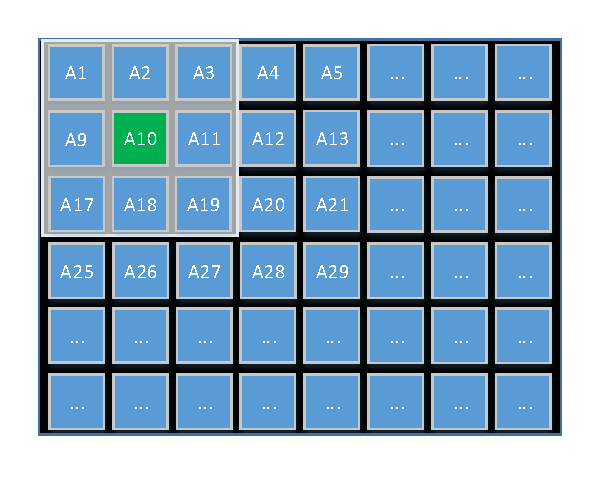
\includegraphics[width=0.5 \textwidth]{picture_example.pdf}
	\caption{Example of sobel matrix calculation}
	\label{fig:pic_matrix}
\end{figure}

\subsection{Border conditions}
\paragraph*{}
Since the Sobel operator is a $3~x~3$ matrix then performing Sobel operation on a pictures border pixel i problematic since the top/bottom row and left/right columns is outside the picture see figure \ref{fig:pic_matrix_border}. There is a couple of ways to handle this. One is to skip calculation of the border which result in a picture of $n-2~x~m-2$ calculated pixels and a untouched border. 

\begin{figure}[H]
	\centering
	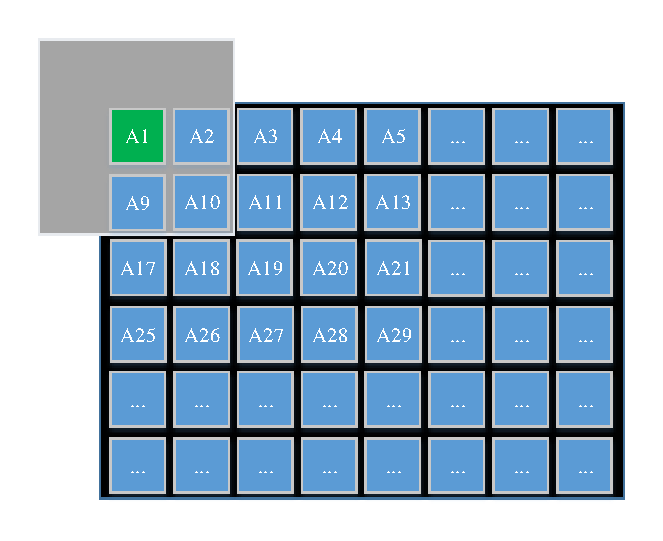
\includegraphics[width=0.5 \textwidth]{picture_example_border.pdf}
	\caption{Example of sobel matrix calculation at borders}
	\label{fig:pic_matrix_border}
\end{figure}

\paragraph*{}
A better and quite simple way to deal with the boarder problem is to make an imaginary or fictive border on the picture. This  can be done by coping the border pixels at the moment they are needed for calculation so that the border pixels give an extra border. The principle is illustrated in figure \ref{fig:pic_matrix_exBorder}.

\begin{figure}[H]
	\centering
	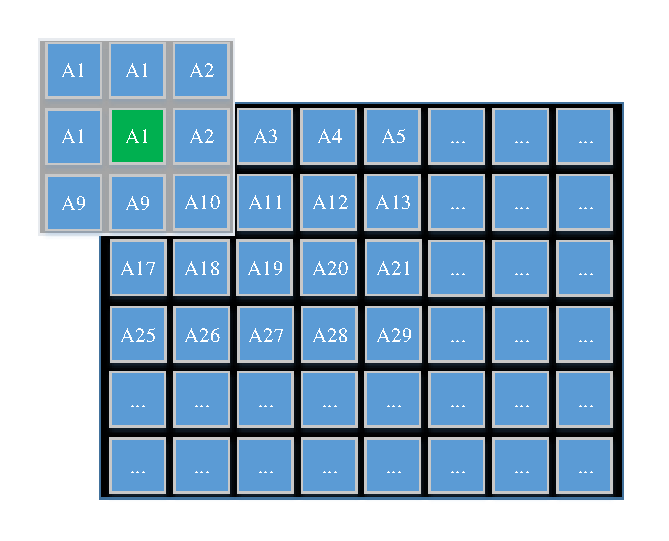
\includegraphics[width=0.5 \textwidth]{picture_example_exBorder.pdf}
	\caption{Example of sobel matrix calculation at borders}
	\label{fig:pic_matrix_exBorder}
\end{figure}  

\subsection{Dynamic range and normalization...}
\paragraph*{}

\section{Accelerator design} 
\label{sec:AccDesign}
\paragraph*{}
This section describes the design of the accelerator and explain how the pixel data is handled when travelling from external memory to the accelerator and back to external memory. 
Because each memory transaction involves two pixels (16bit data width). The proposed design of the accelerator, will process two pixels in parallel, this will increase the throughput without increasing the clock rate. At the same time it also simplifies the data handling, since the accelerator does not need to distinguish between which pixel to process (lower byte or upper byte). The drawback of this parallel approach is that the combinatorial logic that performs the Sobel operation, will be twice as big.

\paragraph*{}
As seen in the previous section \ref{sec:Sobel}, any given pixel, in the output image of the Sobel operator, is a function of the surrounding eight pixels in the input image. This requires that the accelerator is having access to these surrounding pixels, in order to evaluate the Sobel operator. Instead of reading the entire neighborhood from the external RAM, for every single pixel, an obvious improvement is to use a sliding window technique, and thereby reducing the number of memory transactions. If two pixel are to be processed in parallel, a 3x4 sliding window is required. But since the two convolution kernels stretches over three memory addresses, the width of the sliding window must be increased by one pixel, giving a total of 3x5 pixels. This is visualized in figure \ref{fig:shift_register}(a), which shows the two overlapping convolution kernels \emph{(A and B)} and the three memory location they span. \\
Figure \ref{fig:shift_register}(b) shows the proposed sliding window and illustrates how incoming pixels are shifted from right to left.

\begin{figure}[H]
	\centering
	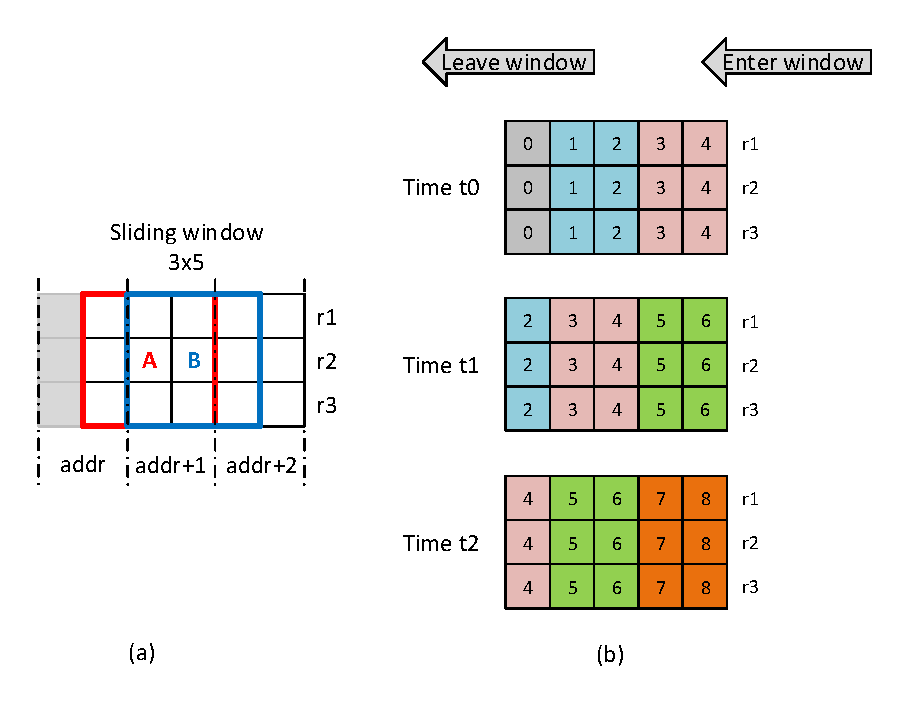
\includegraphics[width=0.9 \textwidth]{SlidingWindow.pdf}
	\caption{3x5 pixel sliding window}
	\label{fig:shift_register}
\end{figure}

\paragraph*{}
A block diagram showing the internal architecture of the accelerator is seen in figure \ref{fig:AccBlockDiagram}. The figure shows how data will flow from memory, over the sliding window through the Sobel operator and back to the memory again. A few control signals to control the memory and sliding window are also depicted in the figure. 

\begin{figure}[H]
	\centering
	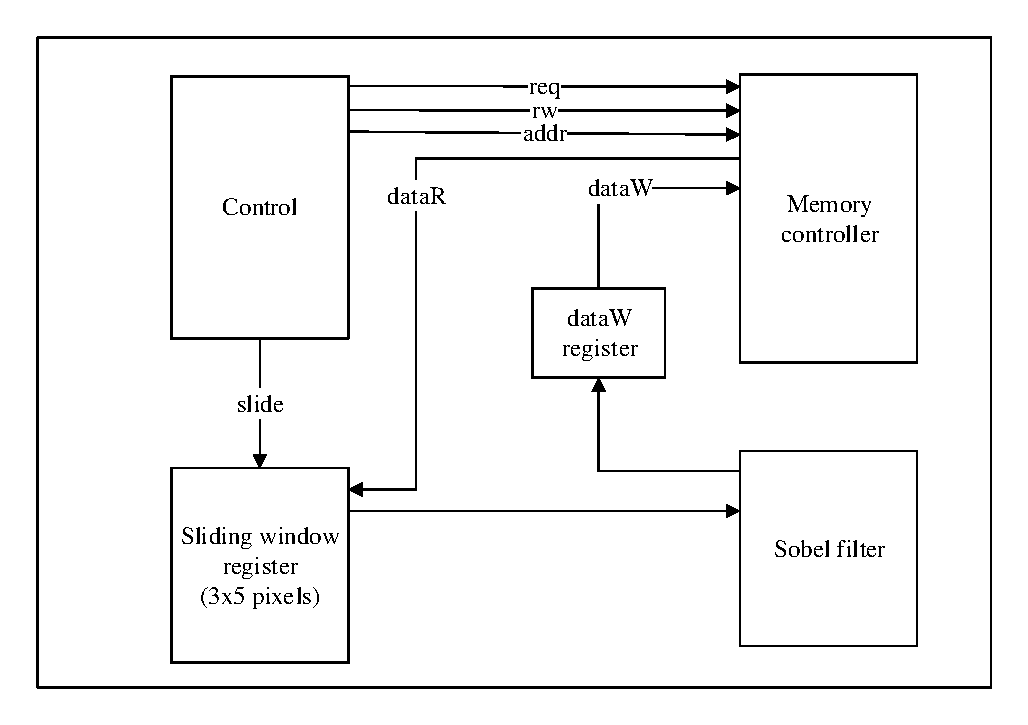
\includegraphics[width=1.0 \textwidth]{Block_diagram_overview.pdf}
	\caption{Internal architecture of the accelerator}
	\label{fig:AccBlockDiagram}
\end{figure}

\paragraph*{}
From the architecture seen in figure \ref{fig:AccBlockDiagram} along with sliding window from figure \ref{fig:shift_register} it is possible to give an initial estimate of the attainable throughput of the accelerator. For each processed pixel pair, the accelerator is required to perform three memory reads and one memory write. Because the memory controller needs to setup the address prior to reading and writing, two extra cycles are to be expected, giving a total of six clock cycles per pixel pair.
With a clock frequency of 12.5 MHz (maximum when the memory is operated in asynchronous mode \cite{Micron:CellularRAM}) this gives a throughput of approximately 4.1M pixel/sec.

\paragraph*{}
Figure \ref{fig:ASM_HW} shows a complete ASMD diagram of the proposed design, that illustrates the operation of the sliding window and details about the image border handling. The ASMD diagram consist of 9 states (\emph{idle, startRow, readSetup, readCenter, readAbove, readBelow, calculateFilter, writeData and doneImage}).
In the \emph{idle} state the accelerator is waiting for the start signal to appear. Once the start signal is detected, the state is changed to \emph{startRow}, in which the current address is initialized to the start of the current image row before entering the next state \emph{readSetup}. In the state \emph{readSetup} the reading of the current address is prepared, this state also handles the sliding of the window as well as the special case for the left and right images borders. 
The state \emph{readCenter} will put the the newly read data into the sliding window and prepare the reading of data located one row above the current position. In case of first row the top image border is handled by reading the current position once more. The state \emph{readAbove} is almost identical to \emph{readCenter}, the difference is that it will prepare the reading of data one row below the current position and that it is handling the bottom image border.
The state \emph{calculateFilter} is performing the Sobel operation and moves the result into a register. The \emph{writeData} state will write the content of the result register to the output image. From the \emph{writeData} state it is possible to enter one of three states. 1)\emph{startRow} in case the end of a row is reached. 2)\emph{doneImage} if the entire image has been processed and 3)\emph{readSetup} in the normal case.
The \emph{writeData} state will increment the current position and current row accordingly. The final state \emph{doneImage} will wait until the start signal is de-asserted before the FSM is returned to the \emph{idle} state.

\paragraph*{}
Because figure \ref{fig:ASM_HW} shows the complete ASMD diagram it is possible to give a fairly accurate estimation of the registers (D-flip flop) required by the suggested design. With knowledge about the Sobel operator (equation \ref{eq:sobel_calc1} and \ref{eq:sobel_abs} ), it the required adders/subtractors can be estimated as well. 
The following table

\begin{table}[h]
	\centering
	\begin{tabular}{lr}
	\hline
	\multicolumn{2}{c}{D-flip flops registers} \\ \hline
	Register						& \# \\ \hline
	State (9 states)				& 4 \\
	3x5 pixel sliding window		& 120 \\
	Sobel result (pixel pair)		& 16 \\
	3 address registers (32 bit)	& 96 \\ \hline
	Total							& 232 \\ \hline
	\end{tabular}
	\caption{Estimated number of registers.}
	\label{tab:designRegisters}
\end{table}


\begin{table}[h]
	\centering
	\begin{tabular}{lr}
	\hline
	\multicolumn{2}{c}{Adders/subtractors} \\ \hline
	Function						& \# \\ \hline
	Address logic (32 bits)			& 6 \\
	Sobel filter (pixel pair, 9- 11 bits)		& 22 \\  \hline
	\end{tabular}
	\caption{Estimated number of Adders and subtractors.}
	\label{tab:designRegisters}
\end{table}
ToDo - Estimating ressource usage ...

\begin{figure}[H]
	\centering
	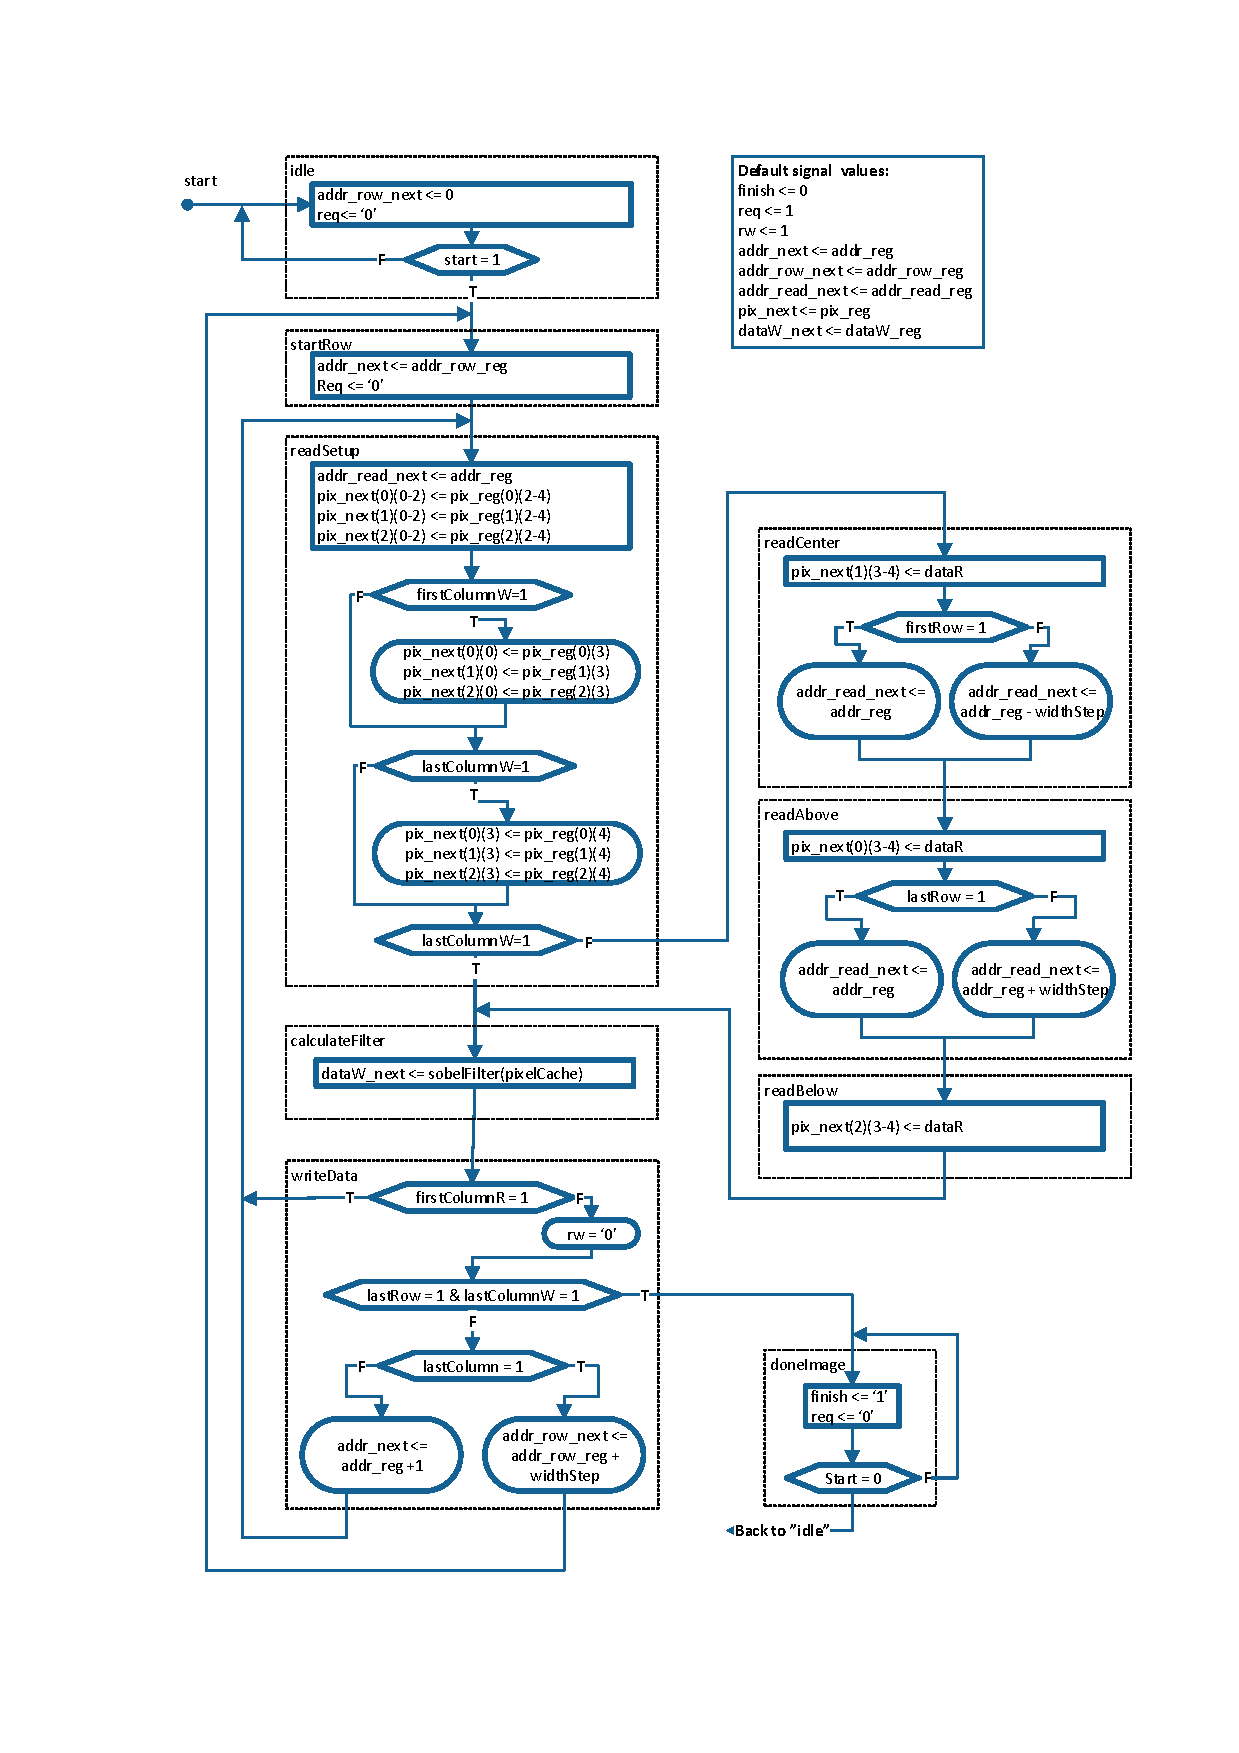
\includegraphics[width=1 \textwidth]{ASM_HWacc.pdf}
	\caption{ASMD chart for the edge detector hardware accelerator}
	\label{fig:ASM_HW}
\end{figure}

\section{Design optimization}
\label{sec:Optimization}
\subsection*{Removing superfluos reads}
\label{sec:memaccess}
\paragraph*{}
Even though the sliding window technique reduces the required memory transactions, the design presented in section \ref{sec:AccDesign}, still need to read every single pixel three times. This is caused by the fact that each row will need data from the row above and below the current position. Since access to the external memory is the main bottleneck in terms of achieving a high throughput, it is desirable to only read the pixel data once. By employing even more caching of data this is indeed possible. Figure \ref{fig:ScanlineBuffers} shows a caching scheme that will assure that data from three consecutive rows are available and ready to enter the sliding window. The cache operates as a delay-line buffer with one tap and contains two full scanlines. Whenever a pixel is read from the external memory it is pushed into one end of the scanline buffer and the tap and end of the delay line buffer will hold pixel data from the two rows just above the pixel being pushed into  scanline buffer. In practise the scanline buffer is implemented as a ring buffer with two pointers addressing the middle-tap and the end position. 
Incoming pixels values will overwrite the end position once it is read.

\begin{figure}[H]
	\centering
	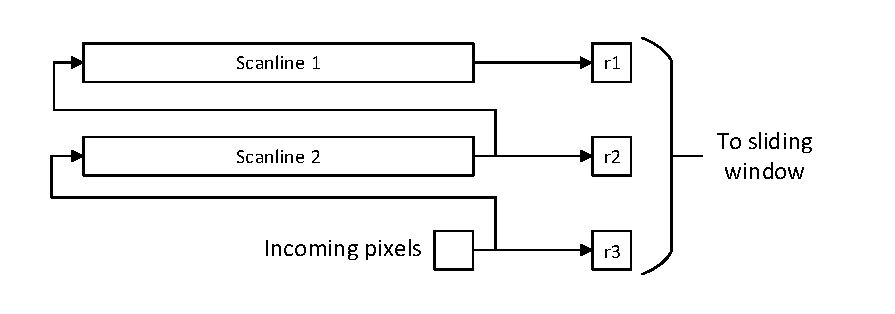
\includegraphics[width=0.9 \textwidth]{ScanlineBuffers.pdf}
	\caption{Scanline buffering of pixel data.}
	\label{fig:ScanlineBuffers}
\end{figure}

\paragraph*{}
The scanline buffer can be implemented as either distributed RAM (using LUT's) or via the block RAM, which is present on most modern FPGA's. Block RAM is usually preferred when larger memories are needed, since the distributed RAM requires more FPGA ressources. The Xilinx Spartan6 chip, used in this assignment, has a true dual ported Block RAM \cite{Xilinx:UG383}, and will be used in the implementation.
Every time the external RAM is being read, the accelerator must perform two reads and one write transaction to the block RAM. Since only two ports are available, it might seems like more than one clock cycle would be required. But because the block RAM is capable of reading the old value prior to writing the new value to a given memory location, all three transactions can be squeezed into one clock cycle.
With the addition of the scanline buffer, the optimized design is able to process a pixel pair in only two clock cycles - one is used when reading from external RAM and one when writing to the external RAM. This is three times faster, compared to a design that only use the sliding window.

\subsection*{Burst mode memory access}
\label{sec:burstmode}
\paragraph*{}
With the scanline buffer introduced above, each pixel is read extacly once. Hence no further throughput optimizations are possible, without increasing the clock rate. The current clock rate of 12.5MHz is limited by the asynchronous mode, that the external memory is operated under. When operating the RAM in synchronous/burst mode, a clock rate of 80MHz is attainable \cite{Micron:CellularRAM}, more than 6 times faster than the asynchronous mode.
However, the burst mode imposes a few challenges to the design, such as increased initial latency (3-4 clock cycles) and a more complex control interface. The initial latency will decrease the throughput, since switching between reading and writing bursts will add a delay to the execution. Therefore the throughput will gain by keeping the bursts as long as possible. On the other hand longer bursts requires larger internal buffering of data waiting to be written back to the RAM. Choosing a burst length of one scanline seems like a good compromise between speed and FPGA resources.

\paragraph*{}
Figure \ref{fig:ASMD_ScanlineBuffers} shows the optimized design, which implements two scanline buffers for the input data. When processing the border pixels, the design is using replication of border pixels as illustrated in figure \ref{fig:pic_matrix_exBorder}. 
Even though the design does not utilize the burst mode, it is prepared for a burst length of one scanline, by using a scanline buffer for queuing the output data, before writing to external RAM.\\
The ASMD diagram is reduced to five states (\emph{idle}, \emph{startRow}, \emph{readData}, \emph{writeData}, \emph{doneImg})

\begin{figure}[H]
	\centering
	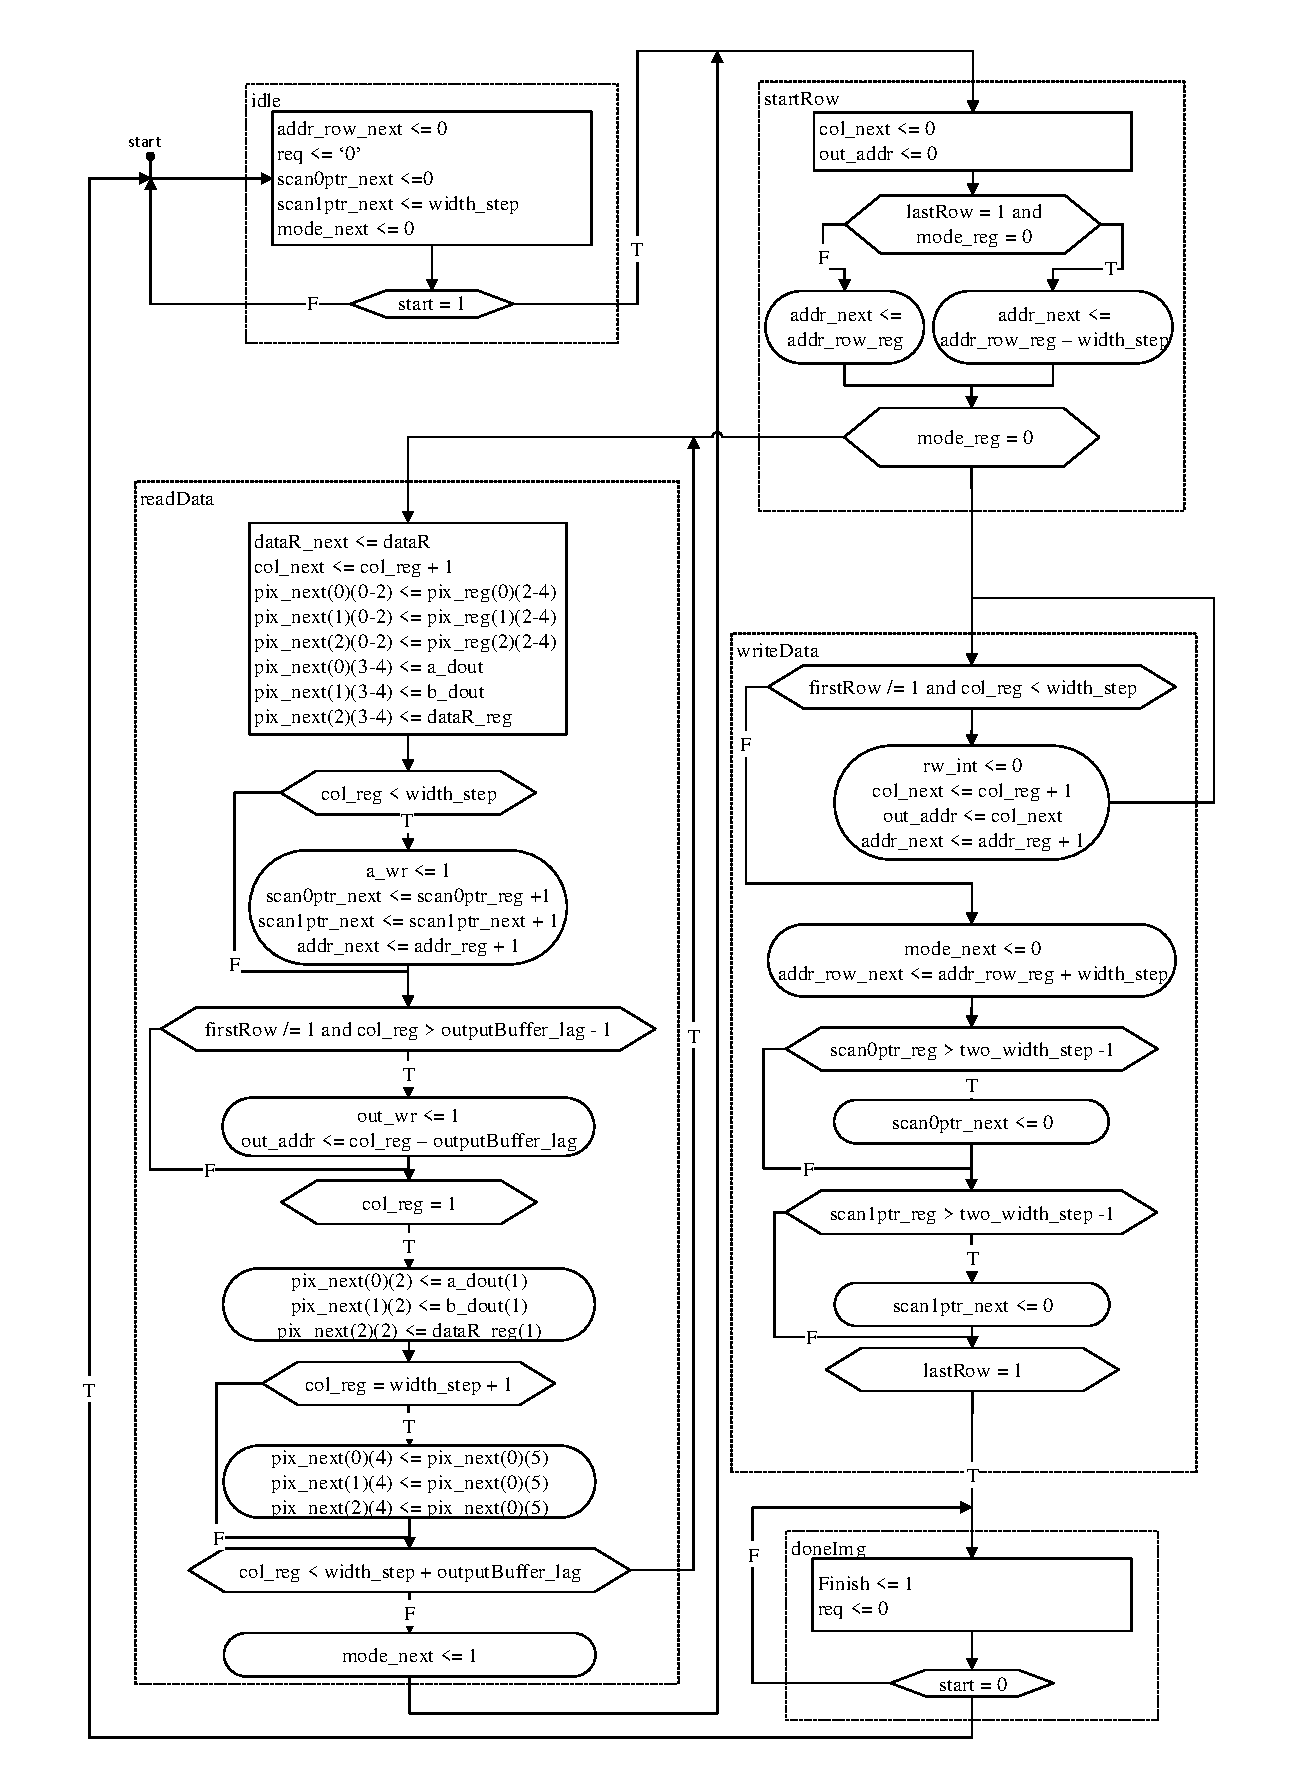
\includegraphics[width=0.9 \textwidth]{ScanlineBuffers_ASM.pdf}
	\caption{Optimized ASMD diagram with scanline buffering of pixel data.}
	\label{fig:ASMD_ScanlineBuffers}
\end{figure}

\chapter{Results}
\label{chap:Results}
\paragraph*{}
From the design given in the previous chapter \ref{chap:theory}, two implementations are created. One without scanline buffers, and the other with scanline buffering. In the following sections, the results from the simulations, synthesis and hardware testing of theses implementations will be presented and discussed. \\
To ensure that the generated results are correct, a Matlab verification script is created (appendix \ref{app:Matlab}). The script contains a reference calculation of the Sobel filter, that mimics the expected and desired operation of the VHDL implementation.
The calculated reference, is subsequently compared with the output image generated by either the simulation or the hardware test.

\textcolor{red}{resource usage slices, LUT's ??}
\section{Implementation of Sobel operator without scanline buffering.}
\paragraph*{}
With the design given in the ASM diagram (figure \ref{fig:ASM_HW} in section \ref{sec:AccDesign}, the VHDL source found in appendix \ref{app:acc2} has been implemented. The implementation have been synthesised, simulated and tested on the \textit{Nexys3 board} and the result is successfully verified by the Matlab verification script.\\
Figure \ref{fig:sum_synthesis_report}, shows an extract from the synthesis report that is generated by the \textit{Xilinx  ISE tool}. The number of inferred D-flip flops are identical to the anticipated values given in table  \ref{tab:designRegisters} and table \ref{tab:designAdders} and the number of adders are two more than the expected number. This discrepancy might be caused by the absolute (\textit{abs()}) functions, which could be constructed from a multiplexer and an adder. 

\begin{figure}[H]
\centering
\small
\begin{BVerbatim}
Summary:
    inferred  31 Adder/Subtractor(s).
    inferred 232 D-type flip-flop(s).
    inferred   3 Comparator(s).
    inferred  59 Multiplexer(s).
    inferred   1 Finite State Machine(s).
\end{BVerbatim}
\caption{Summary of synthesis report ISE project navigator}
\label{fig:sum_synthesis_report}
\end{figure}

From the post place and route report, the maximum frequency is shown in figure \ref{fig:sum_PostPAR_report}. The limiting factor is assumed to by combinatorial circuit that performs the Sobel filter calculation of the sliding window. 

\begin{figure}[H]
\centering
\small
\begin{BVerbatim}
Timing summary:
---------------
Design statistics:
   Minimum period:   9.729ns   (Maximum frequency: 102.785MHz)
\end{BVerbatim}
\caption{Post place and route timing summary.}
\label{fig:sum_PostPAR_report}
\end{figure}

\paragraph*{}
During the implementation and verification of the design, simulations have been performed in ModelSim. Simulations are applied on an image of a roller coaster with an image dimension of $352x288$ pixels, see figure \ref{fig:test_picture_raw}. The image is supplied as part of lab assignment \cite{Sparsoe2014}. The output image from the simulation is seen in figure \ref{fig:test_picture_sobel} and it has been successfully validated by the MATLAB verification script.

\begin{figure}[H]
	\centering
	\begin{subfigure}[b]{0.4\textwidth}
		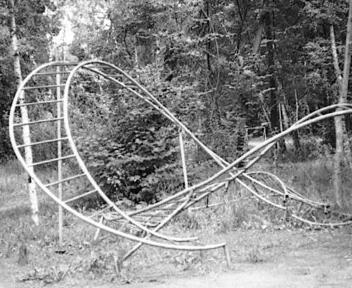
\includegraphics[width=1 \textwidth]{raw.png}
		\caption{Original image before simulation}
		\label{fig:test_picture_raw}
    \end{subfigure}%
        ~ %add desired spacing between images, e. g. ~, \quad, \qquad, \hfill etc. 
    \begin{subfigure}[b]{0.4\textwidth}
    	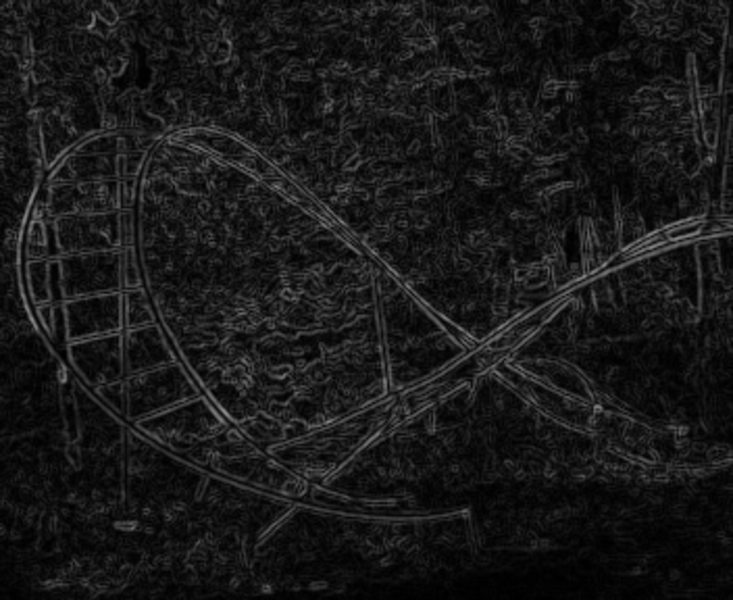
\includegraphics[width=1 \textwidth]{sobel_result.pdf}
    	\caption{Sobel image from simulation}
    	\label{fig:test_picture_sobel}
	\end{subfigure}
	\caption{Simulation result of basic design}
\end{figure}

\paragraph*{}
The simulation is completed in $24.4ms$ which results in a throughput of $40.9$ $frames~pr.~sec$ or $4.15Mpix/sec$, this is in accordance with the estimate done in section \ref{sec:AccDesign}. A part of the simulation waveform can be seen in figure \ref{fig:acc2_waveform}. The waveform depicts one full cycle (6 clock cycles) used when processing a pixel pair. The waveform is annotated to show how the sliding window is shifted, during the state \emph{readSetup} and filled with incoming pixel pairs in the three subsequent states (\emph{readCenter}, \emph{readAbove} and \emph{readBelow}). Finally it shows the result (\emph{dataW}) being written to the output image at an offset memory location (\emph{addr}).

\begin{figure}[H]
	\centering
    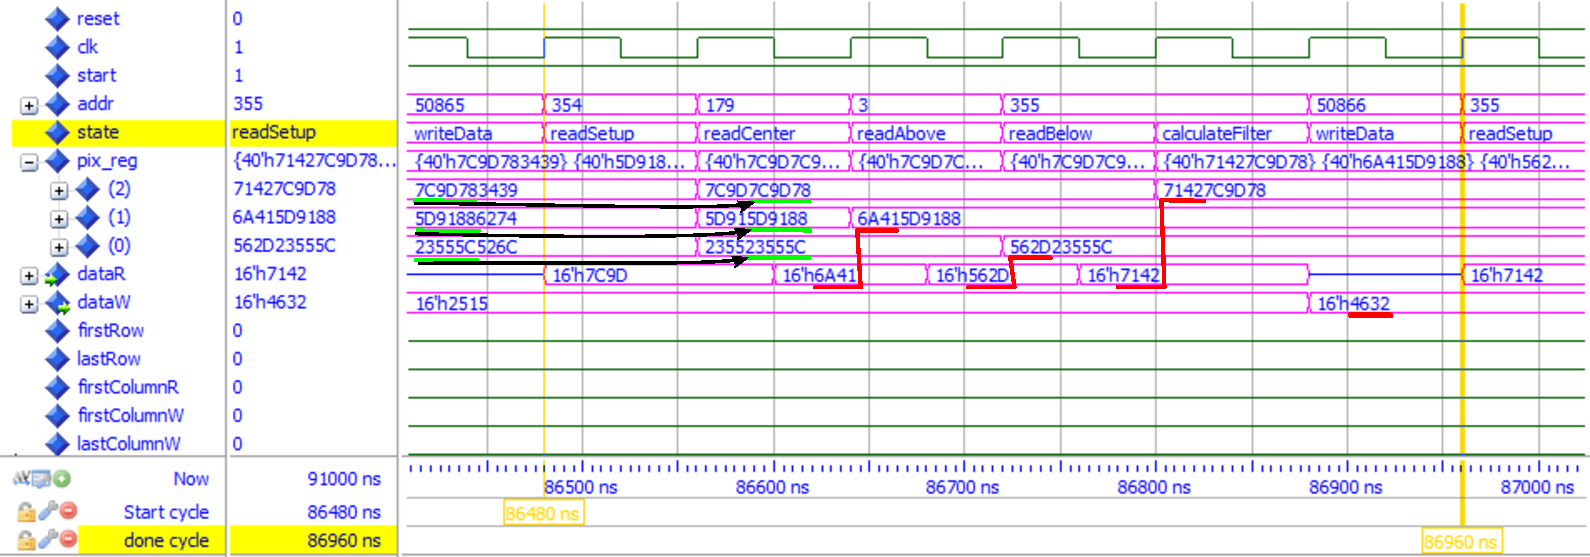
\includegraphics[width=1 \textwidth]{acc2_annotated.pdf}
	\caption{Simulation waveform}
	\label{fig:acc2_waveform}
\end{figure}


\section{Optimization with scanline buffers}
\paragraph*{}
In section \ref{sec:Optimization} a design using scanline buffering was described. This scanline based design has been implemented and synthesized, the results from the simulations and hardware tests have passed the verification script. The VHDL implementation is found in appendix \ref{app:accScanline}. \\
Because this design is using the same circuits for the Sobel calculation and the sliding window, the synthesis report gives roughly the same amount of logic components, See figure \ref{fig:sum_synthesis_report_scan}.
In the synthesis report it is also possible to locate the two dual port block RAM components that is used to form the three scanline buffers. Figure \ref{fig:sum_synthesis_report_ram} list the two inferred block RAMs components. The VHDL implementation of the block RAM can be found in appendix \ref{app:bram}.
    
\begin{figure}[H]
\centering
\small
\begin{BVerbatim}
Summary:
    inferred  34 Adder/Subtractor(s).
    inferred 230 D-type flip-flop(s).
    inferred   5 Comparator(s).
    inferred  75 Multiplexer(s).
    inferred   1 Finite State Machine(s).
\end{BVerbatim}
\caption{Summary of the synthesis report}
\label{fig:sum_synthesis_report_scan}
\end{figure}

\begin{figure}[H]
\centering
\small
\begin{BVerbatim}
Synthesizing Unit <bram_tdp_1>.
    Related source file is "\bram_tdp.vhd".
        DATA_WIDTH = 16
        ADDR_WIDTH = 9
    Found 512x16-bit dual-port RAM <Mram_mem> for signal <mem>.
    Found 16-bit register for signal <b_dout>.
    Found 16-bit register for signal <a_dout>.
    Summary:
	inferred   1 RAM(s).
	inferred  32 D-type flip-flop(s).
Unit <bram_tdp_1> synthesized.

Synthesizing Unit <bram_tdp_2>.
    Related source file is "\bram_tdp.vhd".
        DATA_WIDTH = 16
        ADDR_WIDTH = 8
    Found 256x16-bit dual-port RAM <Mram_mem> for signal <mem>.
    Found 16-bit register for signal <b_dout>.
    Found 16-bit register for signal <a_dout>.
    Summary:
	inferred   1 RAM(s).
	inferred  32 D-type flip-flop(s).
Unit <bram_tdp_2> synthesized.
\end{BVerbatim}
\caption{Inferred Block RAM (synthesis report)}
\label{fig:sum_synthesis_report_ram}
\end{figure}

The maximum clock rate is decreased slightly as seen in figure \ref{fig:sum_ScanPostPAR_report} - A little surprisingly, considering that the combinatorial logic for the Sobel filter is identical to the previos design. One possible explanation, is that the introduction of the block RAMs requires a different place and route layout with longer traces to the output pins (eg. data bus to external RAM).
%I don't think this is reason: The fact that the entire sliding window is updated in one clock cycle, means that the longest combinatorial path for Sobel calculation becomes slighly longer. In the previous design the only one line was updated at a time ...

\begin{figure}[H]
\centering
\small
\begin{BVerbatim}
Timing summary:
---------------
Design statistics:
   Minimum period:  11.134ns   (Maximum frequency:  89.815MHz)
\end{BVerbatim}
\caption{Post place and route timing summary.}
\label{fig:sum_ScanPostPAR_report}
\end{figure}

\paragraph*{}
The simulation of the optimized implementation shows, that by using the scanline buffering described in section \ref{sec:Optimization}, we have managed to reduce the number of memory transactions to the absolute minimum - pixels are only touched once. This is witnessed by a shorter simulation time of $8.29ms$, which is roughly 3 times faster than the previous design, as it was expected. The throughput is now increased to $120$ \textit{frames pr second} or $12.2Mpix/sec$.\\
Figure \ref{fig:acc2_scanWave} shows the waveform from processing a single scanline and it illustrates the interleaving pattern of reading and writing an entire scanline from and to memory.

\begin{figure}[H]
	\centering
    \includegraphics[width=1 \textwidth]{acc2_scan.png}
	\caption{Simulation of scanline based design}
	\label{fig:acc2_scanWave}
\end{figure}
Figure \ref{fig:acc2_scanWaveSlide} depicts how the sliding window is being updated in a single clock cycle and how data is moved to and from the scanline buffers.

\begin{figure}[H]
	\centering
    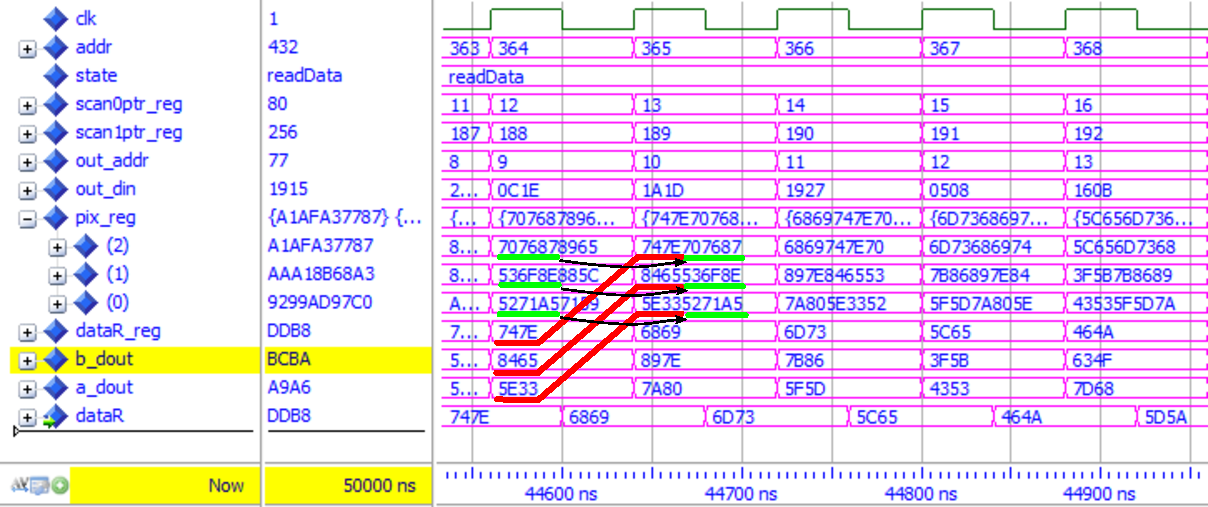
\includegraphics[width=0.8 \textwidth]{acc2_scan_annotated.pdf}
	\caption{Sliding window waveform (scanline version)}
	\label{fig:acc2_scanWaveSlide}
\end{figure}

\section{Burst mode access to external RAM}
\paragraph*{}
Initially we planned for an optimization that would exploit the synchronous mode of the external ram, to achieve the higher clock rate of $80MHz$. Some simulation result are acquired, but we have not been able to provide a working and verified burst mode implementation, within the time frame of this project. Appendix \ref{app:MemBurst} shows an attempt towards, simulating the external memory in continuous burst mode. The implementation consist of a small FSM that simulates the initial latency as well as the row boundary crossing delay that is described in the datasheet \cite{Micron:CellularRAM} of the external memory.
\paragraph*{}
Figure \ref{fig:burst_picture} shows the result obtained from a simulation run, the red markings indicates some of the visible errors in the processed image. The image seen in figure \ref{fig:pic_burst_err} is generated from the MATLAB verification script (app.\ref{app:Matlab}) and gives a more visible representation of the distribution of errors (the black color equals to no error, while the white color indicates an error). From the error image it is observed that the errors occurs systematically a at every $128word$. This gives a strong indication that there is a problem with the row boundary crossing, either in the memory simulation or in the accelerator code.  The burst mode optimization was expected to have a throughput close to $80M pix/sec$ but this is not confirmed, since the implementation has newer been tested in hardware.
     
\begin{figure}[H]
	\centering
	\begin{subfigure}[b]{0.5\textwidth}
		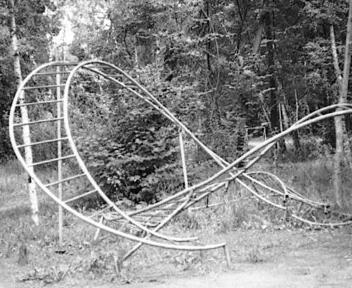
\includegraphics[width=1 \textwidth]{raw.png}
		\caption{Raw image before simulation}
		\label{fig:raw_burst}
    \end{subfigure}%
        ~ %add desired spacing between images, e. g. ~, \quad, \qquad, \hfill etc. 
    \begin{subfigure}[b]{0.5\textwidth}
    	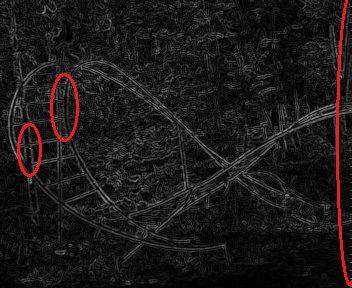
\includegraphics[width=1 \textwidth]{burstResult.png}
    	\caption{After simulation red blobs indicated errors}
    	\label{fig:burst_picture_sobel}
	\end{subfigure}
	\caption{Scanline buffering of pixel data.}
    	\label{fig:burst_picture}
\end{figure}


\begin{figure}[H]
	\centering
	
\includegraphics[width=0.5 \textwidth]{burstErr.png}
	\caption{Image of burst optimization errors}
	\label{fig:pic_burst_err}
\end{figure}
\chapter{Conclusion}
\paragraph*{ }
The aim of this project has been to design and implement a FPGA based hardware accelerator, that performs a Sobel filtering on an image.
The edge detection project has been solved in a structured design process, using RTL methodologies to design block diagrams and  ASMD charts. The general strategy, throughout this project, has been to implement a relatively basic design which is gradually  optimized, to give better performance.
\paragraph*{ }
All the implementations employ a border replication technique, in order to generate an output image with the same dimension as the input image.\\
The first design, which was using a sliding window technique, was able to process $4.1$\textit{M pixel/sec.} Because this design involved four memory transaction per pixel pair this corresponds to data rate of $16.4MB/sec$, when considering both reading and writing from the memory. In asynchronous mode the external memory is capable of a data rate of $25MB/sec.$, which means that this design was not able to use the full potential of the asynchronous memory.\\
In the second design we introduced a scanline buffering mechanism using block RAM, that resulted in a throughput of $12.2M pixel/sec.$ which was a significant improvement. Because this design requires only two memory transactions (read and write) per pixel pair, it equals a data rate of $24.4MB/sec.$ and thereby exploits the full asynchronous bandwidth of the external memory. \\
Our third and last design, which was never fully implemented due to lack of time, involved the synchronous mode of the memory, running at $80MHz$. The theoretically throughput of this design is close to $80M pixel/sec.$ which is equivalent to a data rate of $160MB/sec.$ and thereby utilizing the full bandwidth of the synchronous memory mode.
\paragraph*{ }
For all of the implemented designs, it is clear that the memory access is the dominant limitation in terms of achieving a high throughput. The maximum clock rate of the synthesized implementations are $102.8Mz$ and $89.9MHz$ respectively, which is much higher the asynchronous memory mode but only slightly larger than the synchronous burst mode.


%Overall the project have showed that an edge detection accelerator can indeed be implemented on FPGA how ever with the available hardware in this project it would not be possible to use it for real time calculation on a HD video stream. Since that would require the extern ram to run at $156Mhz$ giving $25.07$ \textit{frames pr. second} for a Full HD resolution.

\newpage
\addcontentsline{toc}{chapter}{Bibliography} 
\bibliographystyle{is-unsrt} % pr�v ogs�: is-unsrt, alpha, plain
\bibliography{biblio/template-bib}

%\newpage\begin{flushright}\begin{flushright}
\chapter*{Appendix}
\addcontentsline{toc}{chapter}{Appendix}

%\chapter{gcd.vhdl}
\newpage
\chapter*{A1	acc2.vhd}
\label{app:acc2}
\addcontentsline{toc}{chapter}{A1	acc2.vhd}			
\lstinputlisting{../task2/acc2.vhd}

\newpage
\chapter*{A2	accScanline.vhd}
\label{app:accScanline}
\addcontentsline{toc}{chapter}{A2	accScanline.vhd}			
\lstinputlisting{../task4/accScanline.vhd}

\newpage
\chapter*{A3	bram\_tdp.vhd}
\addcontentsline{toc}{chapter}{A3	bram\textunderscore tdp.vhd}
\lstinputlisting{../task4/bram_tdp.vhd}

\newpage
\chapter*{A4	acc2 block diagram.vhd}
\addcontentsline{toc}{chapter}{A4 block diagram.vhd}	
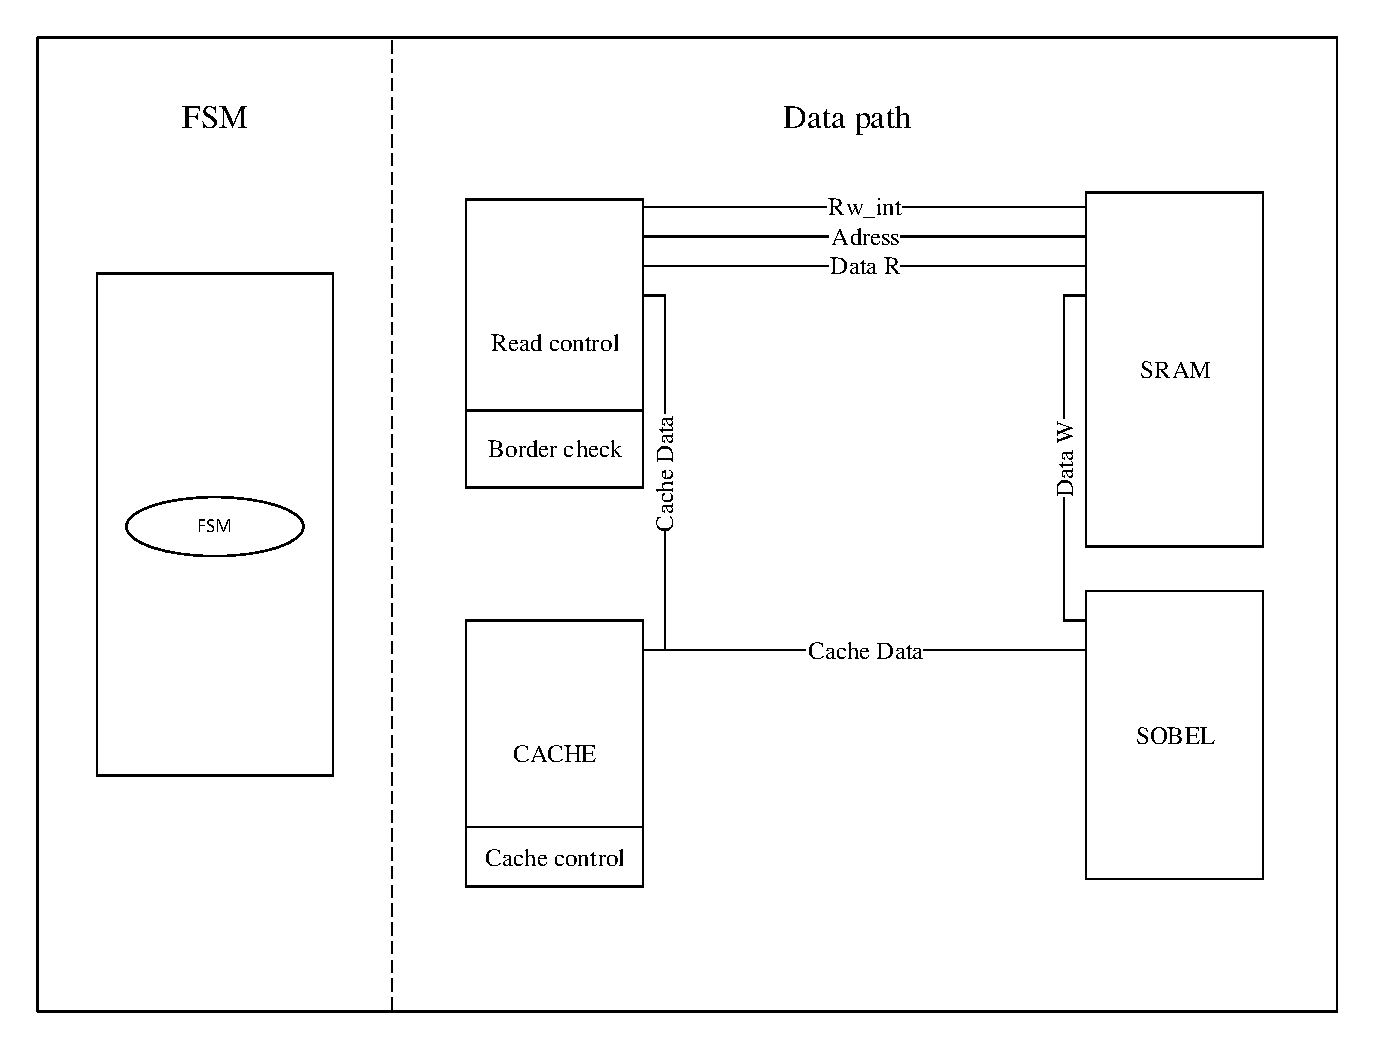
\includepdf[pages={1}]{Block_diagram.pdf}

\newpage
\chapter*{A5	MATLAB verification script}
\label{app:Matlab}
\addcontentsline{toc}{chapter}{A5	MATLAB verification script}
\lstset{language=Matlab} 
\lstinputlisting{../task2/sobel.m}


\end{document}

